\chapter{Materiais e Métodos}
    \label{cap-materiais}

    O método MT proposto por \citeauthor{tikhonov50} \citeyearpar{tikhonov50} e
    \citeauthor{cagniard53} \citeyearpar{cagniard53}, usa das propriedades
    eletromagnéticas para estudar a distribuição de resistividade na crosta, 
    podendo variar a sua investigação em dezenas de metros como dezenas de 
    quilômetros.

    \section{Fundamentos do Método}
	\label{embasamento_teorico}

	As flutuações no campo magnético da Terra e tempestades equatoriais
	geram correntes que penetram no interior da Terra, para 
	simplificar os modelos,	em forma de ondas planas ortogonais, por indução
	geram novas correntes chamadas de correntes 
	telúricas, que trazem informações das características físicas das 
	litologias.

	Uma das características é a modulação da frenquência, causada por
	diferentes tipos de rochas e estruturas, esse fenômeno é diretamente 
	relacionado a resistividade do meio.

	Para construção do método algumas situações de contorno são propostas:
	\begin{enumerate}
	    \item Ondas geradas na ionosfera, distantes o suficientes, penetram ortogonais à superfície
 		da Terra.
	    
	    \item A Terra se comporta como um condutor ôhmico.
	    \item A Terra é considerada um semi-espaço isotrópico.
	\end{enumerate}
	
	A equação \ref{rela_prof_periodo} mostra a relação entre a profundidade
	($\delta_f[m])$, frequência ($f[Hz]$) e a resistividade aparente ($\rho_a[\Omega.m]$), essa 
	profundidade é chamada de \textit{skin-depth} \cite{eletromag8hayt}, e decai com o inverso de $e$.
	\begin{equation}
	 \label{rela_prof_periodo}
	 \delta_\omega = \sqrt{\frac{2}{\omega \mu \sigma}} \longrightarrow \delta_f \approx 500  \sqrt{\frac{\rho_a}{f}}
	\end{equation}
	
	Essa relação mostra que para uma mesma profundidade variando à resistividade
	aparente a frequência é alterada.


    \section{Fundamento Matemático e Leis de Maxwell}
	\label{mat_maxwell}

	Usando as leis de Maxwell \cite{eletromag8hayt} podemos medir os campos elétricos
	e magnéticos separadamente em diferentes componentes e assim unir para obter a 
	função de \textit{skin-depth}.
	
	Os campos podem ser descritos pelas equações a seguir\footnote{Para cargas e correntes livres
	(macroscópica)}:
	    \begin{equation}
		\label{rot_elet_max}
		\nabla \times \vec{\textrm{E}}=-\frac{\partial \vec{\textrm{B}}}{\partial t} 
	    \end{equation}
	    \begin{equation}
		\label{rot_mag_max}
 		\nabla \times \vec{\textrm{H}} = \vec{\textrm{J}} + \frac{\partial \vec{\textrm{D}}}{\partial t}
	    \end{equation}
	    \begin{equation}
 		\nabla \cdot \vec{\textrm{B}} = 0
	    \end{equation}
	    \begin{equation}
 		\nabla \cdot \vec{\textrm{D}} = \rho
	    \end{equation}

	    $\vec{\textrm{E}}$ $\rightarrow$ Campo Elétrico [$V/m$]
	    
	    $\vec{\textrm{B}}$ $\rightarrow$ Campo Magnético [$T$]
	    
	    $\vec{\textrm{H}}$ $\rightarrow$ Campo Magnetizante [$A/m$]
	    
	    $\vec{\textrm{J}}$ $\rightarrow$ Densidade de Corrente [$A/m^2$]
	    
	    $\vec{\textrm{D}}$ $\rightarrow$ Campo de Deslocamento Elétrico [$C/m^2$]
	    
	    $\rho$ $\rightarrow$ Densidade de Carga [$C/m^3$]
	    
	    $t$ $\rightarrow$ Tempo [$s$]

	    Obedecendo as situações de contorno para um meio isotrópico temos as seguintes
	    relações (equações constitutivas):
	    \begin{equation}
	      \label{con_B}
	      \vec{\textrm{B}} = \mu \vec{\textrm{H}}
	    \end{equation}
	    \begin{equation}
	      \label{con_D}
	      \vec{\textrm{D}} = \varepsilon  \vec{\textrm{E}}
	    \end{equation}
	    \begin{equation}
	      \label{con_J}
	      \vec{\textrm{J}} = \sigma \vec{\textrm{E}}
	    \end{equation}
	    
	    $\mu$ $\rightarrow$ Permeabilidade Magnética [$H/m$]
	    
	    $\varepsilon$ $\rightarrow$ Permissividade Elétrica [$F/m$]
	    
	    $\sigma$ $\rightarrow$ Condutividade Elétrica [$S/m$]
	    
	    Cada escalar das equações anteriores são características que dependem do meio 
	    que se propagam.
	    
	    Para a crosta $\mu = 1,2566\textrm{x}10^{-6} H/m$ e $\varepsilon = 8,85
	    \textrm{x}10^{-12} F/m$ esses parâmetros funcionam como tensores em um meio
	    anisotrópico que variam em função do tempo, já considerando para os 
	    trabalhos de investigação o meio supõe-se ser isotrópico, assim, 
	    tornando estáticos os tensores.
	    
	    Outro conceito importante é o tensor Impedância, ele é descrito como uma
	    relação entre os campos elétricos e magnéticos, análogo a Lei de Ohm \cite{eletromag8hayt}
	    que apresentará uma resistência a corrente.
	    
	    \begin{equation}
		\left (\begin{array}{c}
		 \textrm{E}_x\\
		 \textrm{E}_y
		\end{array}\right)
		=
		\left (\begin{array}{cc}
		 \textrm{Z}_{xx} & \textrm{Z}_{xy}\\
		 \textrm{Z}_{yx} & \textrm{Z}_{yy}
		\end{array}\right) \left (\begin{array}{c}
		 \textrm{H}_x\\
		 \textrm{H}_y
		\end{array}\right)
	    \end{equation}
	    
	    \begin{equation}
	     \textrm{E}_x (\omega)=\textrm{Z}_{xx}(\omega) \textrm{H}_{x}(\omega) + \textrm{Z}_{xy}(\omega) \textrm{H}_{y}(\omega)
	    \end{equation}
	    \begin{equation}
	     \textrm{E}_y (\omega)=\textrm{Z}_{yx}(\omega) \textrm{H}_{x}(\omega) + \textrm{Z}_{yy}(\omega) \textrm{H}_{y}(\omega)
	    \end{equation}  
	    
	    Podemos então reescrever as equações \ref{rot_elet_max}
	    e \ref{rot_mag_max} usando as equações constitutivas \ref{con_B}, \ref{con_D}
	    e \ref{con_J}.
	    \begin{equation}
	     \nabla \times \vec{\textrm{E}} = - \mu \frac{\partial \vec{\textrm{H}}}{\partial t} 
	    \end{equation}
	    \begin{equation}
	     \nabla \times \vec{\textrm{H}} = \sigma \vec{\textrm{E}} + \varepsilon \frac{\partial \vec{\textrm{E}}}{\partial t} 
	    \end{equation}
	    O desenvolvimento das equações estão bem descrita no trabalho de \citeauthor{didana2010}\citeyearpar{didana2010}.
	    Apartir do tensor podemos usá-lo para definir a resistividade aparente a partir da equação \ref{rho_a_Z}
	    
	    \begin{equation}
	    \label{rho_a_Z}
	     \rho_a = \frac{1}{\mu_0 \omega } 	\left | \textrm{Z} \right |^2
	    \end{equation}

	   
	   \subsection{Teoria 1D}
	    
	    O modelo de resistividade para a Terra 1D é descrita como a variação da resistividade apenas em profundidade, assim 
	    o tensor impedância é escrito da seguinte forma: 
	    \begin{equation}
	     \textrm{Z}_{1D} = \left (\begin{array}{cc}
	                              0 & \textrm{Z}_{xy}\\
	                              -\textrm{Z}_{xy} & 0
	                              \end{array} \right)
	    \end{equation}
	    Assim a partir das soluções das equações diferenciais temos:
	    \begin{equation}
	     \textrm{Z}_{xy}(\omega) = \frac{\textrm{E}_x(\omega)}{\textrm{H}_x(\omega)} = \frac{\omega \mu_0}{k}
	    \end{equation}
	    Onde $k^2 = i \omega \mu_0 \sigma$. 
	    
	    
	    \subsection{Teoria 2D}
	    O modelo de Terra 2D é caracterizado pelo contato vertical entre dois meios de diferentes resistividades. Se o contato é
	    paralelo ao eixo $x$ então é definido a direção do \textit{strike} no eixo $x$, a direção deve ser paralela ao plano de contato,
	    ou seja, onde a condutividade é constante.% (Figura \ref{fig_strike}).
	    
	    %\begin{figure}[h]
	        %\caption{Modelo de Terra 2D para a resistividade variando na direção $y$}
	        %\begin{center}
	        %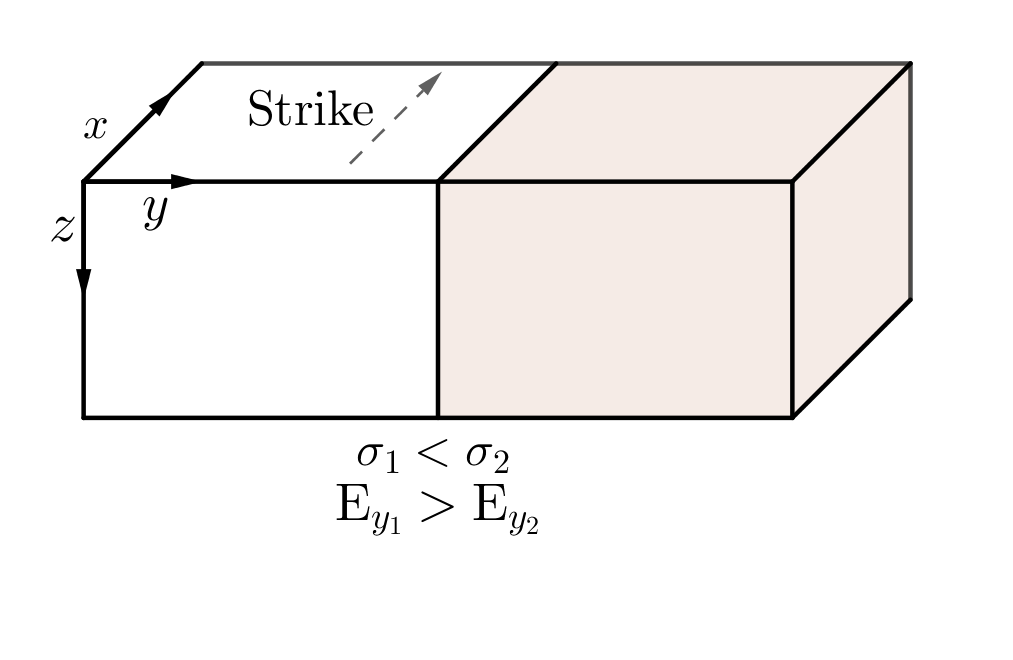
\includegraphics[width=12cm]{fig/Tm_Te.png} 
	        %\end{center}
		%\fonte{Adaptado \cite{didana2010}}
		%\label{fig_strike}
	    %\end{figure}
	    Devido a essa diferença entre as resistividades polarizamos os campos em TE (Transversal Elétrico) e TM (Transversal Magnético).
	    Para esse modelo temos o tensor impedância como:
	    \begin{equation}
	     \textrm{Z}_{2D} = \left (\begin{array}{cc}
	                               0 & \textrm{Z}_{xy} \\
	                               \textrm{Z}_{yx} & 0
	                              \end{array} \right)
	    \end{equation}
	    Assim cada polarização pode ser escrita como:
	    \begin{equation}
	     \textrm{TE} = \left \{ \begin{array}{l}
	            \dfrac{\partial \textrm{E}_x}{\partial y} = \dfrac{\partial \textrm{B}_z}{\partial t} = -i\omega \textrm{B}_z \\
	           \dfrac{\partial \textrm{E}_x}{\partial z} = \dfrac{\partial \textrm{B}_y}{\partial t} = i\omega \textrm{B}_y \\
	           \dfrac{\partial \textrm{B}_z}{\partial y} - \dfrac{\partial \textrm{B}_y}{\partial z} = \mu \sigma \textrm{E}_x 
	           \end{array} \right.
	    \end{equation}
	    \begin{equation}
	     \textrm{TM} = \left \{ \begin{array}{l}
	            \dfrac{\partial \textrm{B}_x}{\partial y} = \mu \sigma \textrm{E}_z \\
	           -\dfrac{\partial \textrm{B}_x}{\partial z} = \mu \sigma \textrm{E}_y \\
	           \dfrac{\partial \textrm{E}_z}{\partial y} - \dfrac{\partial \textrm{E}_y}{\partial z} = i \omega \textrm{B}_x 
	           \end{array} \right.
	    \end{equation}
	    \subsection{Teoria 3D}
	    
	    Na maioria das condições geológicas o modelo se comporta como 3D, isso implica que a 
	    condutividade varia ao longo das três direções ($\sigma = \sigma_{x,y,z}$).
	    
	    A matriz impedância é então calculada com todos os termos, sendo nenhum igual a 0.
	    
	\section{Estrutura do software (RiMT)}
	    \label{rimt}

	    O RiMT será desenvolvido em linguagem Python na sua terceira versão, a
	    linguagem é gratuita o que torna mais fácil o uso no meio acadêmico, todo
	    o código será liberado após a conclusão do projeto sobre os termos da licença
	    GNU. 
	    Os recursos e APIs utilizadas na construção do programação serão:
	    
	    \begin{enumerate}
		\item Kivy 1.10.0 $\rightarrow$ Para a construção da interface gráfica
		\item MatplotLib 2.2.2 $\rightarrow$ Plotagem dos gráficos em conjunto com a API Kivy
		\item Numpy e Scipy $\rightarrow$ Processamento dos dados
		\item Python 3.5 $\rightarrow$ Linguagem base 
	    \end{enumerate}

	    A primeira parte do projeto será a construção da interface usando como \textit{kernel}
	    de processamento os pacotes desenvolvidos pelo grupo GEOMA \citeauthor{geoma} do INPE.
	    
	    Na segunda fase será feita a troca do \textit{kernel} para um novo, escrito
	    somente em Python, essa troca é motivada pelas varias dependências externas que os 
	    pacotes tinham que tornavam o código muito instável e de difícil aprendizagem, porém,
	    escrito somente em python o código terá uma melhor comunicação e tornando também 
	    mais rápido, a partir RiMT o usuário final não terá contato com o as linhas de comando.
	    
	    O programa será desenvolvido para distribuições Linux baseadas no Debian. 
	    
	    Após concluir as duas fases será iniciado o processo de testes com dados
	    sintéticos, e otimização do código. No final serão processados
	    os dados do projeto Estudos geofísicos e tectônicos na Província Borborema,
	    Nordeste do Brasil (MCT/CNPq, 42.0222/2005-7) no nordeste brasileiro, esses dados
	    já foram processados no trabalho de \citeauthor{tese_andrea} de \citeyearpar{tese_andrea}
	    utilizando os pacotes do INPE, os dados serão comparados e analisados.
